\newcommand{\mcQ}{\mathcal{Q}}
\newcommand{\mcS}{\mathcal{S}}
\newcommand{\mcT}{\mathcal{T}}
\newcommand{\nwks}[2]{${#1}$-way, ${#2}$-shot}

\chapter{Few-Shot Learning}\label{chap:fsl}
A good machine learning model often requires training with a large number of samples. Humans, on the contrary, learn new concepts and skills much faster and more efficiently. Children who have only seen cats and birds a few times can quickly tell them apart. People who know how to ride a bike are likely to discover how to ride a motorcycle quickly with little or even no demonstration. Is it possible to design a machine learning model with similar properties - learning new concepts and skills fast with a few training examples? That is essentially what few-shot learning is designed to solve.

Despite notable advances in the field of artificial intelligence, two essential aspects of human conceptual intelligence have consistently eluded machine learning and artificial intelligence (AI) systems. 
First, for most interesting kinds of natural and man-made categories of entities, humans can learn a new concept from just one or a few handful examples, whereas many AI models would require several thousands of examples to perform satisfactorily. 
Second, people learn far richer representations than machines do, even for seemingly simple concepts, and use them for a wide variety of tasks such as creating new entities based on the exemplars, classifying objects into parts, grasping between concepts and parts, and creating new abstract categories (concepts) by combining existing ideas and concepts.
In contrast to this, the best machine learning models and neural networks cannot perform these additional functions using their specialised learnt representations. 
The challenge arises when we wish for AI models to learn new concepts and representations from few examples and ensure that these representations are abstract and flexible.

\section{Formalising the Few-Shot Learning Problem}\label{sec:formalising-fsl}

In a few-shot setting, the model aims to generalise well and quickly enough on a variety of new and potentially unseen tasks after being trained for optimal performance on various learning tasks.
Each task is associated with a dataset $\mathcal{D}$, containing both inputs and true labels. 
The model parameters of an optimal generalisable model are defined as follows:
\begin{equation}
    \symbfit{\theta}^\star = \arg\min_{\symbfit \theta} \mathbb{E}_{\mathcal{D}\sim p(\mathcal{D})} [\mathcal{L}_{\symbfit \theta}(\mathcal{D})]
\end{equation}

First, we look at how \(\mathcal{D}\) is structured in a standard supervised few-shot setting. 
Consider a labelled dataset of size $M$, $\mathcal{D} = \left\{(\symbfit{x}_i, y_i)\, |\, i \in [1,M] \right\}$ of images $\symbfit{x}_i$ and class labels $y_i$. 
This dataset $\mathcal{D}$ is divided into three disjoint subsets: $\left\{\mathcal{D}^\textup{tr}\, \cup\, \mathcal{D}^\textup{val}\, \cup\, \mathcal{D}^\textup{test}\right\} \in \mathcal{D}$, respectively, referring to the training, validation, and test subsets. The validation dataset $\mathcal{D}^\textup{val}$ is used for model selection and the testing dataset $\mathcal{D}^\textup{test}$ for final evaluation. The episodic training is done on a set of tasks $\mathcal{T}_i \sim p(\mathcal{T})$. The tasks are constructed by drawing $K$ random samples from $N$ different classes, which we denote as an ($N$-way, $K$-shot) task. 
Specifically, each task $\mathcal{T}_i$ is made up of a set $\textit{support}$ and a $\textit{query}$ set and each task may also be referred to as an \textquote{episode}. The support set $\mathcal{S}$ contains $K$ samples per class and the query set $\mathcal{Q}$ contains $Q$ samples per class. For a given task, the $NK$ support and $NQ$ query images are mutually exclusive to evaluate the generalisation performance of the model.
\begin{figure}[ht]
    \centering
    \captionsetup{justification=centering}
    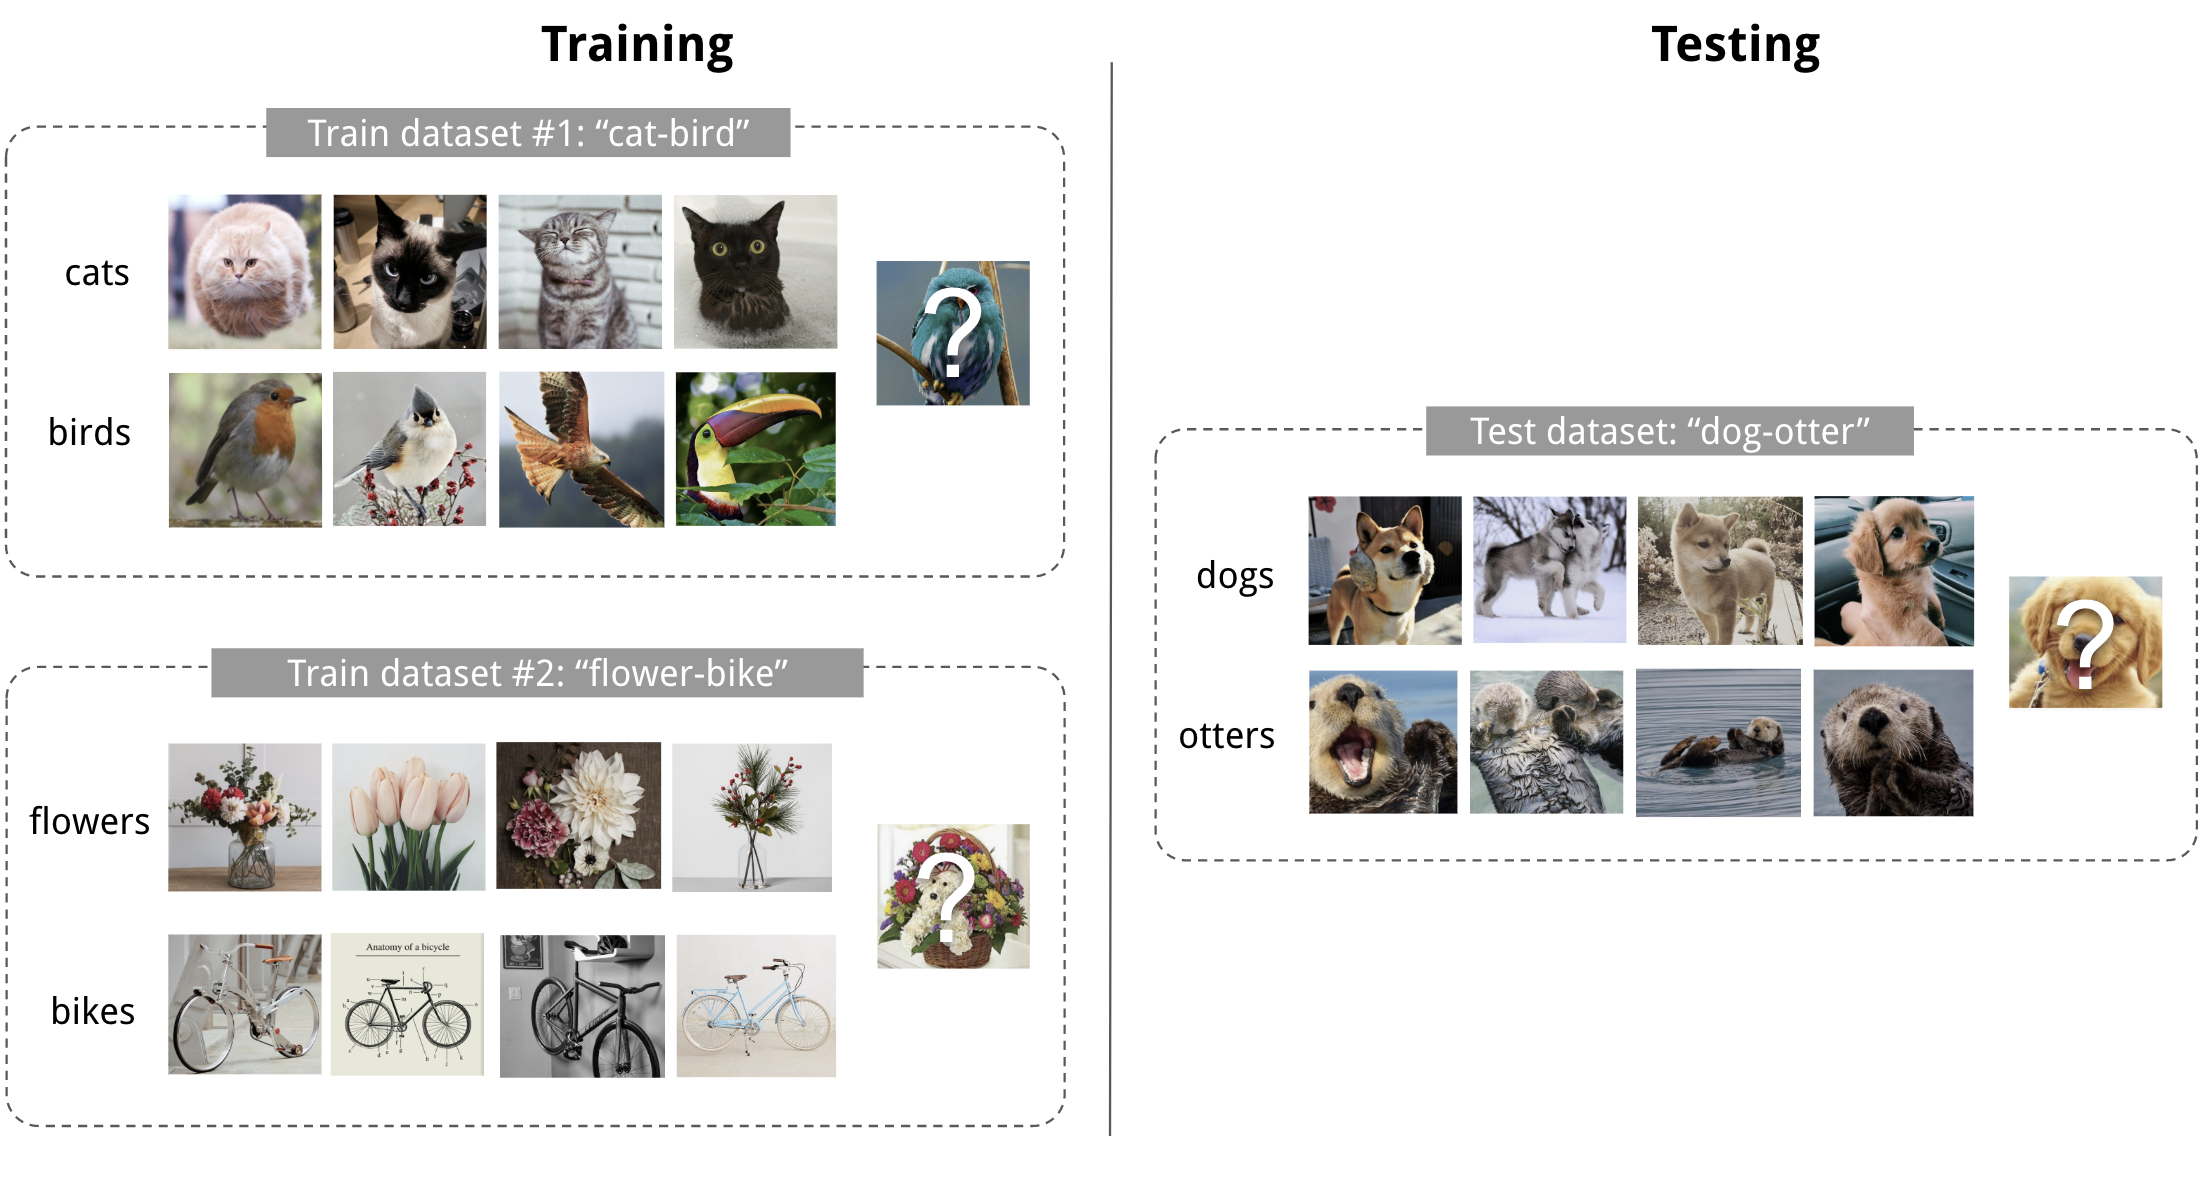
\includegraphics[width=\linewidth]{chapters/assets/fsl/few-shot-classification.png}
    \caption{An example of (\nwks{2}{4}) image classification.}
    \label{fig:fsl-tasks}
\end{figure}

In most training routines, tasks are randomly sampled from a task distribution according to the (\nwks{N}{K}) setting, and then the model parameters are updated by backpropagation after each task.
This comprises one episode. The model is expected to quickly learn the optimal parameters from the $NK$ support data points and apply the learnt weights to classify the $NQ$ unlabelled query data points, on which the performance is evaluated.
\Cref{fig:fsl-tasks} shows (\nwks{2}{4}) training tasks, it must be noted that even during testing (downstream classification task) the model is presented with tasks that are in the same (\nwks{2}{4}) form as the training tasks.

\section{Model Agnostic Meta Learning (MAML)}\label{sec:maml}
\textbf{Meta-learning} is most commonly understood as learning to learn, which refers to the process of improving a learning algorithm over multiple learning episodes and was first proposed by \textcite{schmidhuber:1987:srl}. In contrast, conventional ML improves model predictions over multiple data instances. 
During base learning, an \emph{inner} learning algorithm solves a task such as image classification, defined by a dataset and objective. During meta-learning, an \emph{outer} algorithm updates the inner learning algorithm such that the model it learns improves an outer objective.
Learning episodes of the base task, namely tuples of image $\bfitx_i$ and associated label $y_i$, can be seen as providing the instances needed by the outer algorithm to learn the base learning algorithm

\begin{wrapfigure}{r}{0.25\linewidth}
    \centering
    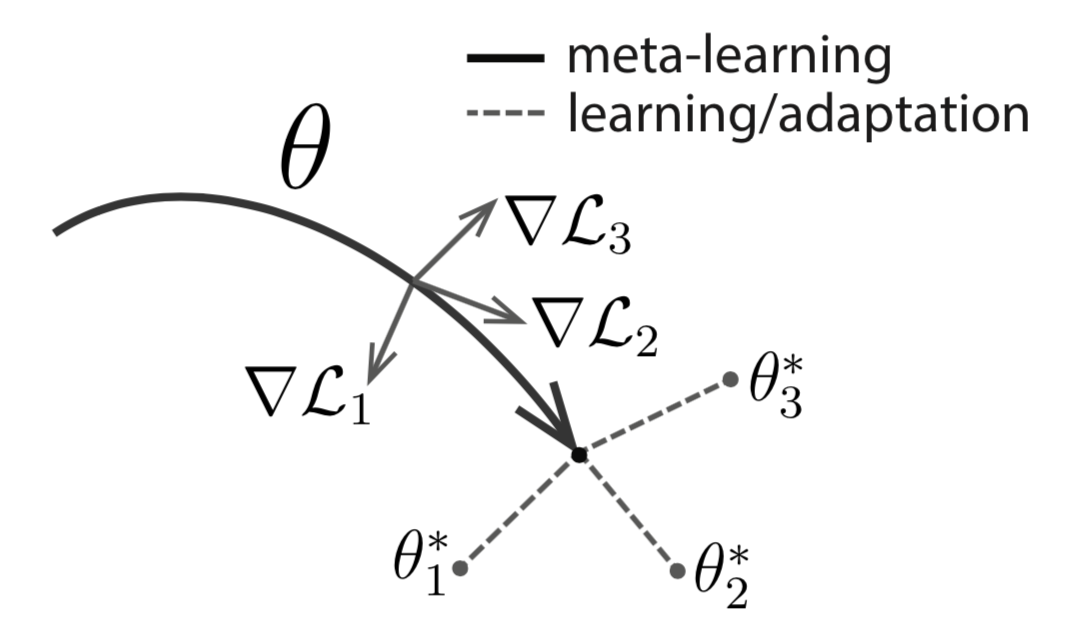
\includegraphics[scale=0.23]{chapters/assets/fsl/maml.png}
    \caption{MAML tries to find optimal generalised weights, by first finding optimal weights in the inner learning phase.}
    \label{fig:maml}
\end{wrapfigure}
MAML is a gradient based \textbf{meta learning} method. It is a technique that works with any model which learns through gradient descent. It trains a model to find an optimal set of weights that can be quickly adapted to a new task, through a few gradient descent steps. The meta-learner tries to find an initial set of weights that are not only useful for adapting to various problems, but also can be adapted quickly (in a small number of steps) and efficiently (using only a few examples).

In \Cref{fig:maml} we are trying to find a set of parameters $\theta$ that can be easily adapted. MAML optimises for a set of parameters so that when a gradient step is taken with respect to a particular task $\mcT_i $ (the grey lines), the parameters are close to the optimal parameters $\theta^*_i$ for task $\mcT_i$.

This approach is fairly simple and has several advantages. It does not make any assumptions about the form of the model. It is quite efficient - no additional parameters are introduced for meta-learning, and the learner strategy uses a known optimisation process (gradient descent), rather than having to come up with one from scratch. It can also be easily applied to a number of domains, including classification, regression, and reinforcement learning. However, it can be computationally expensive due to the use of higher-order gradients, as we will see.

Given a task and its associated support and query sets $\langle S, Q \rangle$, we can update the model parameters by one or more gradient descent steps (the following example only contains one step):
\begin{equation}
    \theta^\prime_i = \theta - \eta \nabla_\theta\mathcal{L}^{(0)}_{\mcT_i}(f_\theta)
    \label{eqn:one-task-maml}
\end{equation}
where $\mathcal{L}^{(0)}$ is the loss computed using the task with id $(0)$.

\begin{equation}
    \begin{aligned}
            \theta^* 
            &= \arg\min_\theta \sum_{\mcT_i \sim p(\mcT)} \mathcal{L}_{\mcT_i}^{(1)} (f_{\theta'_i}) = \arg\min_\theta \sum_{\mcT_i \sim p(\mcT)} \mathcal{L}_{\mcT_i}^{(1)} (f_{\theta - \alpha\nabla_\theta \mathcal{L}_{\mcT_i}^{(0)}(f_\theta)}) & \\
            \theta &\leftarrow \theta - \beta \nabla_{\theta} \sum_{\mcT_i \sim p(\mcT)} \mathcal{L}_{\mcT_i}^{(1)} (f_{\theta - \alpha\nabla_\theta \mathcal{L}_{\mcT_i}^{(0)}(f_\theta)}) & \scriptstyle{\text{; updating rule}}
    \end{aligned}
    \label{eqn:maml-update-rule}
\end{equation}

The update rule in \Cref{eqn:one-task-maml} only optimises for one task. To achieve a good generalisation on a variety of tasks, we would like to find the optimal $\theta^\star$ so that the task-specific fine-tuning is more efficient.
Now, we sample a new task with id $(1)$ to update the outer objective (also called the meta-objective).
For the outer objective we use the meta update rule given in \Cref{eqn:maml-update-rule}, the task specific parameters are used to calculate the loss on a query set, based on this loss the meta update is applied. The meta update is essentially unrolling the task-specific optimisation and backpropagating through the optimisation process.The loss, denoted as $\mathcal{L}^{(1)}$, depends on the task $(1)$. The superscripts in $\mathcal{L}^{(0)}$ and $\mathcal{L}^{(1)}$ only indicate different tasks and refer to the same loss objective for the same task.
For more details, please refer to \parencite{Finn2017Model-agnosticNetworks}.


\section{Prototypical Networks}\label{ssec:protonets}

Prototypical networks are a type of\textbf{metric learning} models. The core idea in metric learning is similar to nearest neighbours algorithms ($k$-NN classifier and $k$-means clustering) and kernel density estimation. The goal of Metric Learning is to learn a representation function that maps objects into an embedded space. The distance in the embedded space should preserve the objects' similarity; similar objects get closer, and dissimilar objects get far away. The similarity metric is learnt by a kernel function $\mathscr{k}_{\symbfit{\theta}}$, parameterised by $\symbfit{\theta}$. The distances measured by the kernel function are converted into probabilities on a set of labels $y_i \forall i$ by means of a softmax or sigmoid function. Both $\ccclr$ and $\samptr$ make use of prototypical networks for classification because this method is simple yet robust as evidenced by the performance of $\ccclr$ and $\samptr$.

Prototypical networks learn a non-linear function, $f_{\symbfit \theta}$, that maps the input to a feature vector in an embedding space (or representation space) using a parameterised neural network in a supervised manner. The embeddings of the $K$-shots for each of the $N$-classes are averaged in order to compute the \textbf{class prototypes}. Traditionally, a \textit{prototype} is an entity that is the archetypal form of \textquote{something}, for example, Boeing $777$\footnote{\url{https://www.boeing.com/commercial/777/}} jets are prototypes of modern large passenger jets.
Here, a class prototype $\symbfit{c}_k$ plays a similar role; it is a feature vector that is defined for every class $k \in \mathcal{C}$, as the mean vector of the embedded support set samples in class $k$, and is calculated as:
\begin{equation}
    \symbfit{c}_{k}=\frac{1}{|\mcS_{k}|} \sum_{({\symbfit x}_i, y_i) \in {\mcS_k}} f_{\symbfit \theta}(\symbfit{x}_{i}).
    \label{eqn:fsl-proto-calc}
\end{equation}

\begin{figure}[ht]
    \centering
    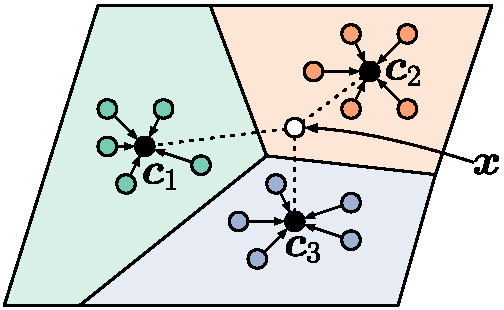
\includegraphics[scale=0.85]{chapters/assets/fsl/prototype_fewshot_v3.pdf}
    \caption{Few-shot prototypes $\symbfit{c}_k$ are computed as the mean of embedded support examples for each class. Image sourced from \parencite{Snell2017PrototypicalLearning}.}
    \label{fig:protonets}
\end{figure}

The distribution over classes for a given query input $\symbfit{x}$ is a softmax over the inverse of the distances between the embedding of the query data and the prototype vectors:
\begin{equation}
    P(y=k\vert\symbfit{x})=\operatorname{softmax}\left(-d(f_\theta(\symbfit{x}), \symbfit{c}_k)\right) = \frac{\exp(-d(f_\theta(\symbfit{x}), \symbfit{c}_k))}{\sum_{k^\prime \in \mathcal{C}}\exp(-d(f_\theta(\symbfit{x}), \symbfit{c}_{k^\prime}))}
    \label{eqn:fsl-proto-classification}
\end{equation}
where $d$ can be any distance function as long as it is a differentiable operation to allow for gradient-based learning. In the original work, \textcite{Snell2017PrototypicalLearning} use the Euclidean distance metric.

Learning is carried out by minimising the negative log likelihood $J(\symbfit{\theta})$ and performing stochastic gradient descent over the same to update the kernel's parameters $\symbfit{\theta}$:
\begin{equation}
    J(\theta)=-\log P_{\symbfit \theta}(y=k \vert \symbfit{x}).
\end{equation}


\section{Unsupervised Few-Shot Learning}\label{sec:u-fsl}

So far, we have only discussed few-shot learning in a supervised setting. However, a more challenging scenario is the unsupervised setting. Recall that the dataset in the supervised setting is given as \(\mathcal{D} = \left\{(\symbfit{x}_i, y_i)\, |\, i \in [1,M]\right\}\) which implies that we have the true class labels $y_i$ available to us during training time. In the unsupervised setting we no longer have access to the true labels during the training period. 

Then a question naturally arises: How do we create valid tasks (see \Cref{sec:formalising-fsl}) if we do not have access to the true labels? This is an important question, consider \Cref{fig:fsl-tasks} where we illustrate (\nwks{2}{4}) shots, we see that each of the $2$ classes have exactly $4$ samples. Tasks like this would be taxing to create without labels. To overcome this, there are a few creative methods that we shall discuss in the following sections.

\subsection{CACTUs}\label{ssec:ufsl-cactus}
CACTUs was one of the first methods aimed at solving the unsupervised few-shot learning problem \parencite{Hsu2018UnsupervisedMeta-Learning}. CACTUs uses MAML as part of its training mechanism to obtain a generalisable model. CACTUS also retains the episodic task-based training strategy introduced by MAML \parencite{Finn2017Model-agnosticNetworks}. Unlike MAML, however, a major aspect of CACTUs is dedicated to a clever \textbf{task creation} technique, as it cannot be fed standard tasks, as discussed above.
\begin{figure}[ht]
    \centering
    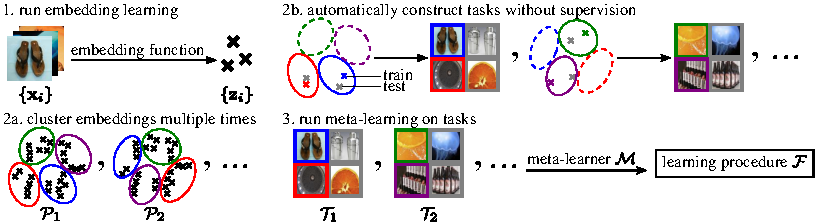
\includegraphics[width=\linewidth]{chapters/assets/fsl/cactus.pdf}
    \caption{Illustration of CACTUs. }
    \label{fig:cactus}
\end{figure}
The idea of CACTUs is to use a separate embedding learning algorithm $\mathcal{E}$ on $\bfitx_i \in \mathcal{D}$ to produce embeddings $\{\symbfit{z}_i\}$. CACTUs then uses $k$-means clustering on $\{\symbfit{z}_i\}$ $P$ times in order to generate a set of partitions $\mathcal{P}_P = \{\mathcal{C}_P\}$. CACTUs can technically make use of any self-supervised (more generally, unsupervised) representation learning methods to train $\mathcal{E}$. \textcite{Hsu2018UnsupervisedMeta-Learning} choose to use DeepCluster \parencite{caron2018deep}, BiGAN \parencite{berthelot2018understanding}, ACAI \parencite{donahue2016adversarial}, and InfoGAN \parencite{chen2016infogan}. 

CACTUs then samples a partition $\mathcal{P}$ randomly from the set of parititons $\{\mathcal{P}_P\}$, following which a cluster $\mathcal{C}_n$ is randomly sampled from the partition $\mathcal{P}$. The cluster sampling process is carried out $N$ times for each of the classes desired in a (\nwks{N}{K}) task. Similarly, the process is repeated for $Q$ query images. Finally, the randomly sampled support and query images are used to create a \textbf{synthetic} task that is fed into MAML.

A major concern here is that CACTUs is dependent on bigger models, like AlexNet \parencite{AlexNet2012}, using powerful self-supervised learning methods on a small dataset like \miniImagenet{}. The embeddings (representations) generated by this larger model are then used to create synthetic tasks to train a more simpler Conv$4$ architecture. It has been known for quite some time that larger models consistently offer better performance and representations \parencite{Dosovitskiy2020, He2015}, these better representations indirectly aid a smaller Conv$4$ to learn better.

\subsection{UMTRA} \label{ssec:umtra}

\begin{figure}[ht]
    \centering
    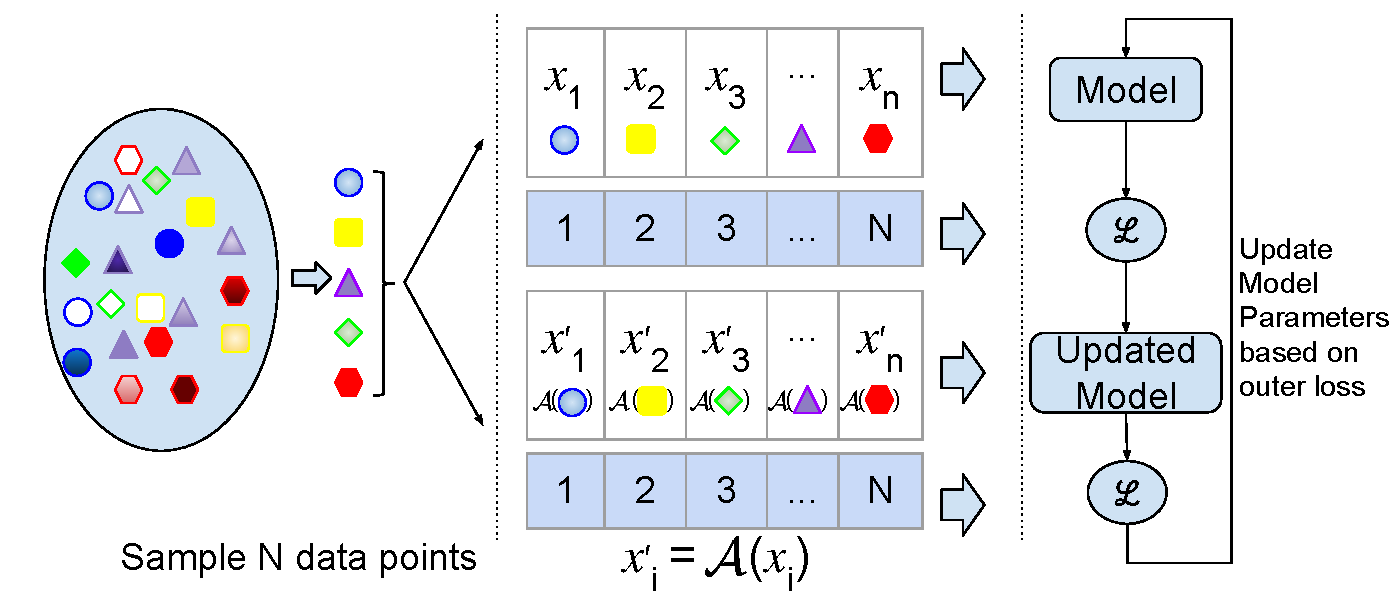
\includegraphics[width=\linewidth]{chapters/assets/fsl/UnsupervisedMetaTraining3.pdf}
    \caption{umtra}
    \label{fig:umtra}
\end{figure}

\subsection{ProtoTransfer}\label{ssec:prototransfer}

\begin{figure}
%\captionsetup[subfigure]{labelformat=empty}
\centering
\begin{minipage}{\textwidth}
  \centering
  \setlength{\unitlength}{1cm}
  %\thicklines
    \begin{picture}(13.5,5)
    \put(0,0){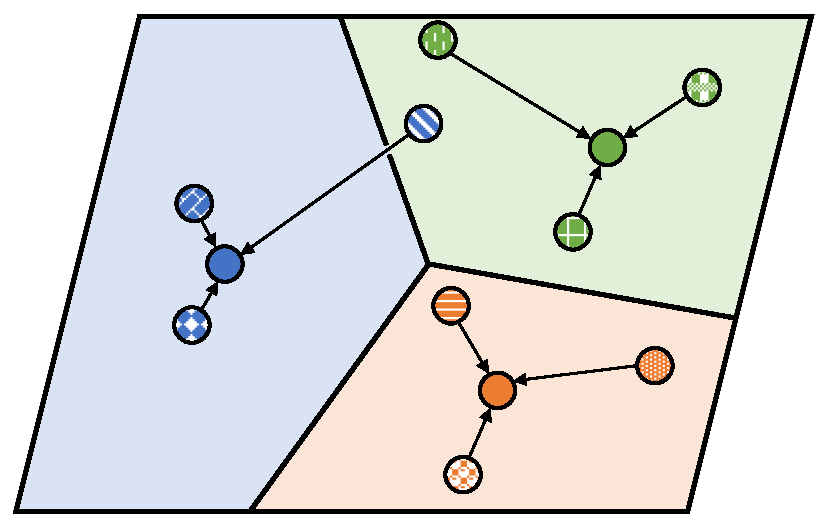
\includegraphics[scale=0.45]{chapters/assets/fsl/selfsupproto.pdf}}
    %\put(-4,-1){{ $3$-simplex}}
    \put(7.3,0){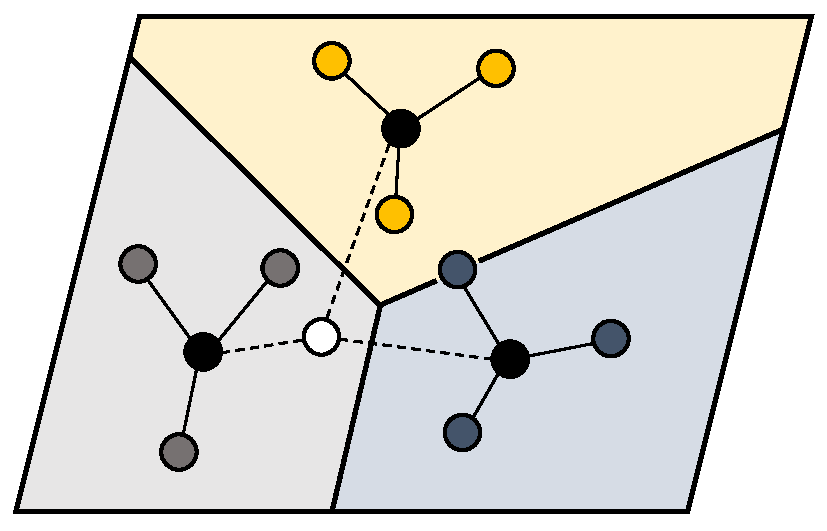
\includegraphics[scale=0.45]{chapters/assets/fsl/protofinetune.pdf}}
    \put(1.9,1.9){$\scriptstyle f_\theta(\symbfit{x}_i)$}
    \put(1,1.2){$\scriptstyle f_\theta(\tilde{\symbfit{x}}_{i,1})$}
    \put(1,2.8){$\scriptstyle f_\theta(\tilde{\symbfit{x}}_{i,2})$}
    \put(3.1,2.7){$\scriptstyle f_\theta(\tilde{\symbfit{x}}_{i,3})$}
    
    \put(4.8,2.8){$\scriptstyle f_\theta(\symbfit{x}_{2})$}
    
    \put(3.9,.8){$\scriptstyle f_\theta(\symbfit{x}_{1})$}
    %\put(0,0){\circle{0.1}}
    %\put(0,5){\circle{0.1}}
    %\put(7,0){\circle{0.1}}
    %\put(7,5){\circle{0.1}}
    \put(10.5,2.9){$\scriptstyle \symbfit{c}_{1}$}
    \put(8.4,1.1){$\scriptstyle \symbfit{c}_{2}$}
    \put(11.3,1.1){$\scriptstyle \symbfit{c}_{3}$}
    
    \put(9.3,1.1){$\scriptstyle f_\theta(\symbfit{q})$}
    \end{picture}\\
    \hspace{-.2cm}(a) Self-Supervised Prototypical Pre-Training \hspace{.8cm} (b) Prototypical Fine-Tuning \& Inference
  %\caption{(a) Self-Supervised Prototypical Pre-Training \hspace{2cm} (b) Prototypical Fine-Tuning \& Inference}
  \label{fig:sub2}
\end{minipage}
\caption{Self-Supervised Prototypical Transfer Learning. (a): In the embedding, original images $\symbfit{x}_i$ serve as class prototypes around which their $Q$ augmented views $\tilde{\symbfit{x}}_{i,q}$ should cluster. (b): Prototypes $\symbfit{c}_{n}$ are the means of embedded support examples for each class $n$ and initialize a final linear layer for fine-tuning.
An embedded query point $\symbfit{q}$ is classified via a softmax over the fine-tuned linear layer.}
\label{fig:algorithm}
\end{figure}


% \subsection{Matching Networks}\label{ssec:matching-nets}
% Like any network involved in a classification problem, matching networks also learn a classifier that we will call $\mathscr{v}_{\mcS}$ for any given support set $\mcS$. This classifier defines a probability distribution on the output labels $\symbfit{y}$ given a query sample $\bfitx$. Similar to prototypical networks, the classifier output is defined as a sum of support samples per class, weighted by an attention kernel $a(\bfitx, \bfitx_i)$ the value of which is proportional to the similarity between query $\bfitx$ and support sample $\bfitx_i$.

% Matching networks differ from other metric learning approaches by the fact that they condition not only the classification strategy on the entire support set (attention kernel computed over the entire support set), but also the embedding function. \textcite{Vinyals2016MatchingLearning} argue that methods in which the cosine similarity is applied to simply compute the nearest neighbour are myopic in the sense that each element $\bfitx_i$ gets embedded by $g_\theta(\bfitx_i)$ independently of other elements in the support set $\mathcal{S}$. Thus, \textcite{Vinyals2016MatchingLearning} argue that the images in $\mathcal{S}$ should be able to modify how the test image $\bfitx$ is embedded using $f_{\symbfit \theta}$.

% For a more intuitive understanding, suppose that we have two inputs in the support set $x_i, x_j$ that are extremely similar.
% When using the encoder $g_\theta(x_i, S)$, it would be helpful if the function that embeds $x_j$ would be dependent on the input $x_i$ and also change based on the output embedding of $x_i$. 

% \begin{figure}[ht]
%     \centering
%     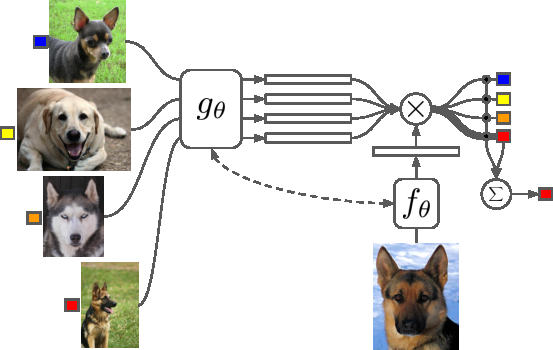
\includegraphics[width=\linewidth]{chapters/assets/fsl/matching_nets.pdf}
%     \caption{Illustration of the working of Matching Nets. Image borrowed from \parencite{Vinyals2016MatchingLearning}.}
%     \label{fig:maching_nets}
% \end{figure}

%Let us denote the training data of size $D$ as $\mathcal{D}_{\textup{tr}} = \{({\symbfit x}_i, y_i)\}_{i = 1}^{D}$ with $({\symbfit x}_i, y_i)$ representing an image and its class label, respectively. In the pre-training phase, we take $L$ random samples from $\mathcal{D}_{\textup{tr}}$ and augment each sample $A$ times by randomly sampling augmentation functions $\zeta^a(.), \forall a \in [A]$ from the set $\mathcal{A}$. This results in a mini-batch of size $B = (A + 1)L$ total samples. Note that in the unsupervised setting we have no access to the data labels in the pre-training phase. Next, we fine-tune our model episodically \cite{Vinyals2016MatchingLearning} on a set of randomly sampled tasks $\mathcal{T}_i$ drawn from the test dataset $\mathcal{D}_{\textup{tst}} = \{({\symbfit x}_i, y_i)\}_{i = 1}^{D^\prime}$ of size $D^\prime$. The tasks $\mathcal{T}_i$ are constructed by drawing $K$ labeled and $Q$ unlabeled random samples from $N$ different classes, which is called an ($N$-way, $K$-shot) task, and denoted by $(N, K)$. The $NK$ labeled samples make up the support set $\mathcal{S}$, from which the model learns, and the other $NQ$ unlabeled samples make up the query set $\mathcal{Q}$, on which the model is evaluated
